\documentclass{article}
\usepackage{amsmath,amssymb,setspace,verbatim,graphicx,enumerate,enumitem}
\usepackage[top=1in,bottom=1in,left=1in,right=1in,head=0.5in,foot=0.5in]{geometry}
\usepackage{caption}
\usepackage{mathtools}
% \usepackage{subcaption}
% \usepackage{subfig}
% \usepackage{subfloat}
% \usepackage{tabularx}
\usepackage{mdframed}
\usepackage{amsthm}

\newtheorem*{theorem}{Theorem}

\newenvironment{Rcode}% environment name 
{%begin code
    \begin{mdframed}
    \#R code
    \begin{small}
}
{%end code
    \end{small}
    \end{mdframed}
}

\newenvironment{console}% environment name 
{%begin code
    \begin{mdframed}
    \#Console
    \begin{small}
}
{%end code
    \end{small}
    \end{mdframed}
}

\begin{document}
\title{STDA Homework 2}
\author{Seokjun Choi}
\date{May 1, 2020}
\maketitle

\textbf{Note:}
You can get full code files at my github page: Visit https://github.com/letsjdosth/SpaTempoDA \\
See "HW2" directory.

Because I provide the full code separately, in this report 
I will show only must-necessarily key code blocks, instead of bringing the whole, verbose code.

\section{Problem 1}
\textbf{
We will carry out profile log-likelihood methods based on the provided code (HW2.R).
You may use the same simulation settings as in the provided code.
\begin{itemize}
    \item Visualize profile log-likelihood of $\rho$ for $[0.005, 0.5]$ interval.
    \item Obtain MLE for $\rho, \beta, \sigma^2$.(Hint: you may use optimize or optim function in R to get MLE of $rho$.)
\end{itemize}
}

In the given setting, We want to get the MLE from the log-likelihood function,
\[l(\beta,\sigma, \rho) \propto -\frac{1}{2} log|\Sigma(\sigma^2,\rho)| - \frac{1}{2}(Y-X\beta)'\Sigma(\sigma^2,\rho)^{-1}(Y-X\beta) \]
where $\Sigma(\sigma^2,\rho)_{i,j}= \frac{|s_i-s_j|\rho}{\sigma^2}$, the exponential covariance.
To simplify the optimization problem of the log-likelihood, I do profiling $\beta$ and $\sigma^2$,
since exponential covariance function has easy form to profile $\sigma^2$.

First of all, fix $\rho$ and calculate MLE for $\beta, \sigma^2$ analytically under the $\rho$.
Then, we get
\[\hat{\beta}(\rho) = (X'\Sigma(\rho)^{-1}X)^{-1}X'\Sigma(\rho)^{-1}Y\]
\[\hat{\sigma}^2(\rho) = \frac{1}{n} (Y-X\hat{\beta}(\rho))'\Sigma(\rho)^{-1}(Y-X\hat{\beta}(\rho))\]
Plug them to the original log-likelihood function. Then we get the profile log-likelihood which depend only on $\rho$.
It may, however, not be complicate to optimize the likelihood analytically so that I optimize it numerically.
The result is summarized by below plot which illustrates the profile likelihood function with respect to $\rho$ 
on the range $[0.005, 0.5]$ and its critical point.

\begin{figure}[hh]
    \centering
    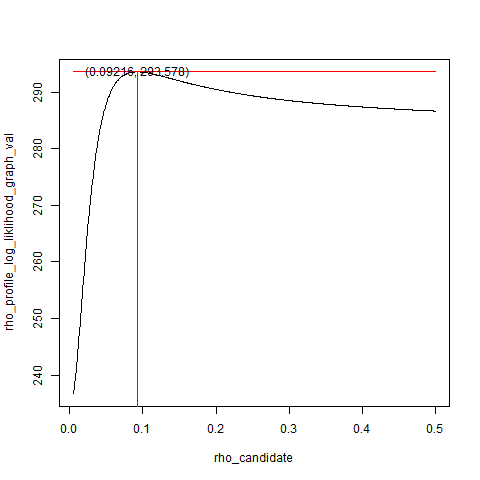
\includegraphics[height=7cm]{prob1_rho_profile_log_likelihood.png}
    \caption{the profile log-likelihood of $\rho$}
\end{figure}

The value $\rho$ which maximize the likelihood is about
\[\hat{\rho}_{P-MLE} = 0.09216\]

Next, using this $\rho_{P-MLE}$, calculate $\hat{\beta}(\hat{\rho}_{P-MLE})$ and $\hat{\sigma}^2(\hat{\rho}_{P-MLE})$.
Then, we get
% write the values!
\[\hat{\beta}_{P-MLE} = 
\begin{bmatrix}
    -0.03921947 & 1.21942596 & 0.94645748
\end{bmatrix} \]
\[\hat{\sigma}^2_{P-MLE} = 0.09971098\]
These are what we want.


\section{Problem2}
\textbf{
Following the model in page 7 of STDA4 slide, based on the provided code, do below.
\begin{itemize}
    \item Clearly write down conditional distribution for $\beta, \tau, \sigma^2, \eta_{obs}$.
        (You no need to write down for $\rho$ because there is no closed form.)
    \item Clearly write down pseudo-code of the Metropolis-Gibbs sampler.
    \item Replicate the results: (1) Provide MCMC diagnostic plots for $\beta, \tau, \sigma^2$.
        (2) Provide prediction maps (both predictive posterior mean and standard deviation).
\end{itemize}
}
For my convenience, I deal with $\tau^2$ instead of $\tau$, and drop the 'obs' subscript of $\eta_{obs}$.

Let's get conditional distributions for $\beta, \tau^2, \sigma^2, \eta_{obs}$.
For beginning, we should get a joint posterior of the parameters.

By Bayes theorem, the pdf of the joint posterior becomes
\[f(\eta,\sigma^2,\tau^2,\rho^2)
    \propto f(Y|\eta,\sigma^2,\tau^2,\rho)f(\eta|\sigma^2,\tau^2,\rho)f(\sigma^2)f(\tau^2)f(\rho)\]
\[\propto N(\eta,\tau^2I) * GP(X'\beta, \sigma^2 K(\rho))
    * N(m_\beta,v_\beta) * InvGamma(a_\sigma^2, b_\sigma^2) * InvGamma(a_\tau^2, b_\tau^2)
    * Gamma(a_\rho, b_\rho) \]
\[\propto (\frac{1}{\tau^2})^n e^{-\frac{(Y-\eta)^2}{2\tau^2}}
    * (\frac{1}{(\sigma^2 K(\rho))^{\frac{1}{2}}})^n e^{-\frac{(\eta-X'\beta)^2}{2\sigma^2 K(\rho)}}
    * e^{-\frac{(\beta-m_\beta)^2}{2v_\beta^2}}
    * (\sigma^2)^{-a_{\sigma^2}-1} e^{-\frac{b_{\sigma^2}}{\sigma^2}}
    * (\tau^2)^{-a_{\tau^2}-1} e^{-\frac{b_{\tau^2}}{\tau^2}}
    * \rho^{a_{\rho}-1} e^{-b_{\rho}\rho}
    \]
where $K(\rho)=K(.,.,\rho)$ is exponential term of exponential covariance.

To get conditional distribution of each parameter, I just read terms of the joint distribution
including the wanted parameter. 

Note that, after mixing two gaussian kernel with respect to a parameter,
we get another gaussian kernel, with variance which is by inverting original two variances (or simply say, 'precisions') and adding them together,
and mean which is by weighted average of original two means using precisions as weights. Or,
\[e^{-\frac{(X-m_1)^2}{2v_1^2}} * e^{-\frac{(X-m2)^2}{2v_2^2}}
    \propto e^{-\frac{(X-(\frac{m_1}{v_1^2} + \frac{m_2}{v_2^2})/(\frac{1}{v_1^2} + \frac{1}{v_2^2}))^2}{2(\frac{1}{v_1^2}+\frac{1}{v_2^2})}}\]

\clearpage
(\textbf{NOTE}: At below, I use the expression like $\frac{1}{A}$ for a matrix $A$, although it is not correct. 
Precisely, I have to use $A^{-1}$ instead of $\frac{1}{A}$.
However, I keep using the fractional notation, for intuition and showing how two means and variances are mixed together more directly.)

for $\eta$,
\[f(\eta|\beta,\sigma^2,\tau^2,\rho,Y) \propto e^{-\frac{(\eta - (\frac{y}{\tau^2} + \frac{X'\beta}{\sigma^2 K(\rho)}) / (\frac{1}{\tau^2}+\frac{1}{\sigma^2 K(\rho)}))^2}{2(\frac{1}{\tau^2}+\frac{1}{\sigma^2 K(\rho)})}}
\]
\[\sim N(\frac{\frac{y}{\tau^2} + \frac{X'\beta}{\sigma^2 K(\rho)}}{\frac{1}{\tau^2}+\frac{1}{\sigma^2 K(\rho)}}, \frac{1}{\tau^2}+\frac{1}{\sigma^2 K(\rho)})\]

for $\beta$,
\[f(\beta|\eta,\sigma^2,\tau^2,\rho,Y) \propto e^{-\frac{(\beta - (\frac{X\eta}{\sigma^2 K(\rho)} + \frac{m_\beta}{v_\beta}) / (\frac{X^2}{\sigma^2 K(\rho)}+\frac{1}{v_\beta})^2}{2(\frac{X^2}{\sigma^2 K(\rho)}+\frac{1}{v_\beta})}}
\]
\[\sim N(\frac{\frac{X\eta}{\sigma^2 K(\rho)} + \frac{m_\beta}{v_\beta}}{\frac{X^2}{\sigma^2 K(\rho)}+\frac{1}{v_\beta}}, \frac{X^2}{\sigma^2 K(\rho)}+\frac{1}{v_\beta})\]

for $\sigma^2$,
\[f(\sigma^2|\eta,\beta,\tau^2,\rho,Y) \propto (\sigma^2)^{-(a_{\sigma^2}+\frac{n}{2})-1} e^{\frac{1}{\sigma^2}(\frac{(\eta - X'\beta)^2}{2K(\rho)}+b_{\sigma^2})}
\]
\[\sim InvGamma(a_{\sigma^2}+\frac{n}{2}, \frac{(\eta - X'\beta)^2}{2K(\rho)}+b_{\sigma^2})\]

for $\tau^2$,
\[f(\tau^2|\eta,\beta,\sigma^2,\rho,Y) \propto (\tau^2)^{-(a_{\tau^2}+\frac{n}{2})-1} e^{\frac{1}{\tau^2}(\frac{(Y - \eta)^2}{2}+b_{\tau^2})}
\]
\[\sim InvGamma(a_{\tau^2}+\frac{n}{2}, \frac{(Y - \eta)^2}{2}+b_{\tau^2})\]


Since we have conditional distributions of parameters except $\rho$,
we are ready to generate samples of the joint posterior using Metropolis-Gibbs sampler.
Pseudo code is here.
\begin{mdframed}
    \begin{small}
        \begin{verbatim}
Y = data; (eta[0], beta[0], sigma_sq[0], tau_sq[0], rho[0]) = initial_values
for i in 1:sample_num:
    new_eta = random_sample_from_eta's_conditional_posterior(
        beta[i-1], sigma_sq[i-1], tau_sq[i-1], rho[i-1], Y)
    new_beta = random_sample_from_beta's_conditional_posterior(
        new_eta, sigma_sq[i-1], tau_sq[i-1], rho[i-1], Y)
    new_sigma_sq = random_sample_from_sigma_sq's_conditional_posterior(
        new_eta, new_beta, tau_sq[i-1], rho[i-1], Y)
    new_tau_sq = random_sample_from_tau_sq's_conditional_posterior(
        new_eta, new_beta, new_sigma_sq, rho[i-1], Y)
    (eta[i],beta[i],sigma_sq[i],tau_sq[i]) = new_eta, new_beta, new_sigma_sq, new_tau_sq

    proposed_rho = proposal_distribution_of_rho(rho[i-1])
    #(comment: commonly, this part is implemented by log version, worrying for underflow.)
    MH_ratio = unnormalized_joint_posterior(proposed_rho)*proposal_pdf(rho[i-1]|proposed_rho)/
        (unnormalized_joint_posterior(rho[i-1])*proposal_pdf(proposed_rho|rho[i-1]))
    unif_random_sample = random_sample_from_uniform(0,1)
    if MH_ratio > unif_random_sample:
        rho[i] = proposed_rho
    else:
        rho[i] = rho[i-1]
Do:
    diagnostics (get summary statistic, traceplot, acf plot, acc-rate of rho, ESS and so on.)
    If needed, cut burn-in period and do thinning.
        \end{verbatim}
    \end{small}
\end{mdframed}

\clearpage
Just running the given "STDA4.R", we can replicate the posterior samples of our model.
Here are the diagnostic plots.

\begin{figure}[!h]
    \centering
    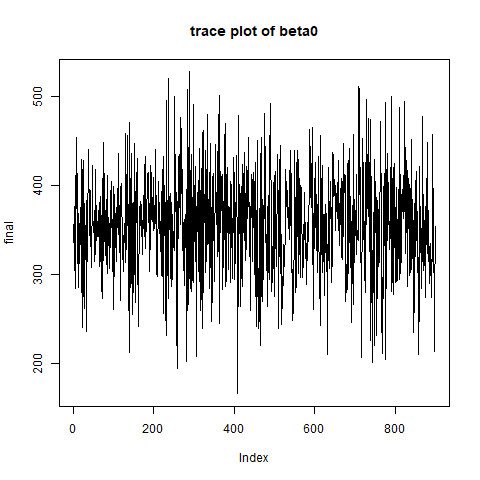
\includegraphics[width=4cm]{prob2_beta0_traceplot.png}
    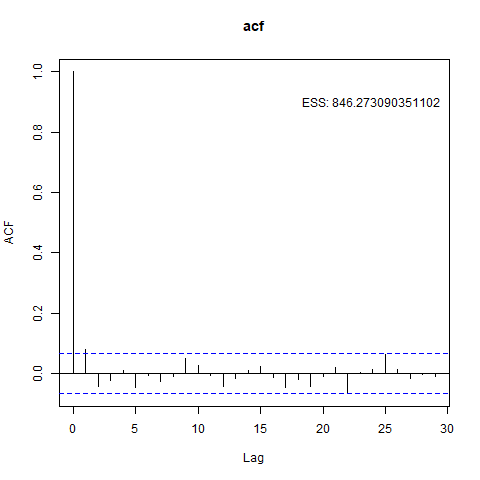
\includegraphics[width=4cm]{prob2_beta0_acf.png}
    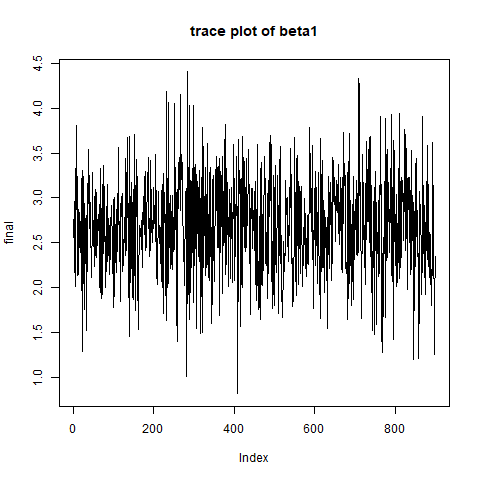
\includegraphics[width=4cm]{prob2_beta1_traceplot.png}
    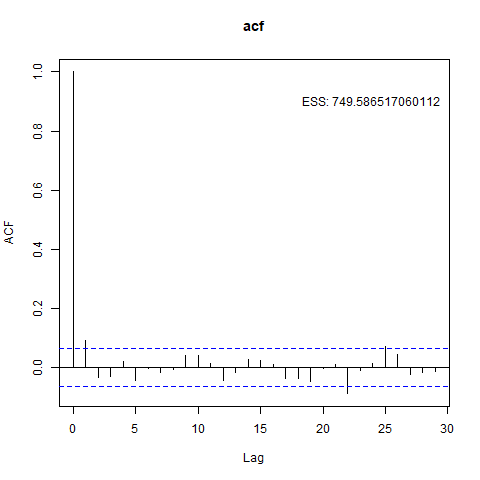
\includegraphics[width=4cm]{prob2_beta1_acf.png} \\
    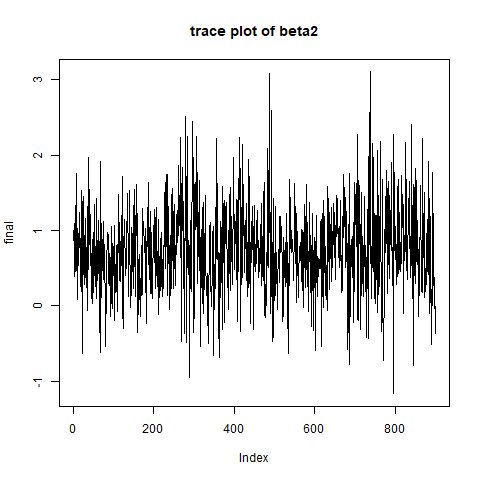
\includegraphics[width=4cm]{prob2_beta2_traceplot.png}
    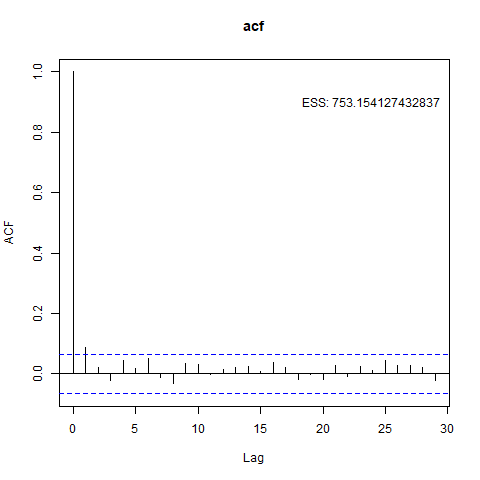
\includegraphics[width=4cm]{prob2_beta2_acf.png}
    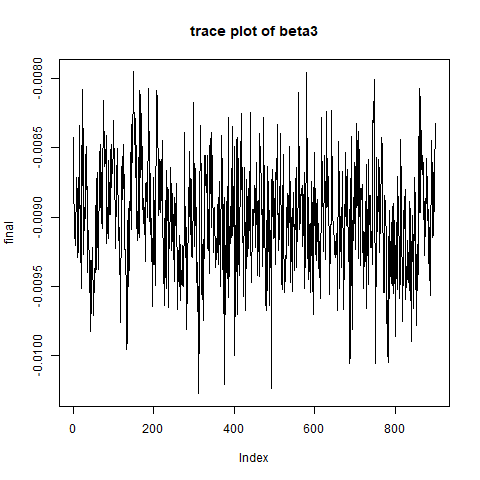
\includegraphics[width=4cm]{prob2_beta3_traceplot.png}
    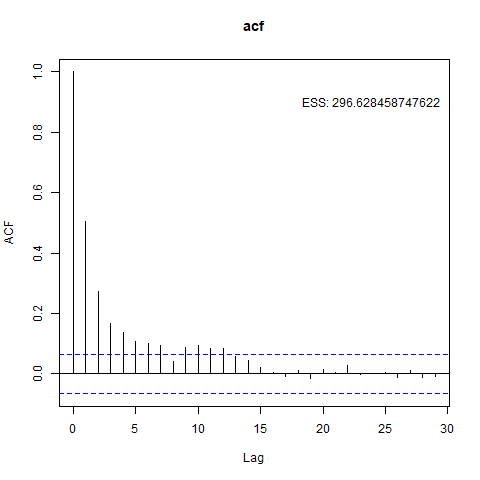
\includegraphics[width=4cm]{prob2_beta3_acf.png}\\
    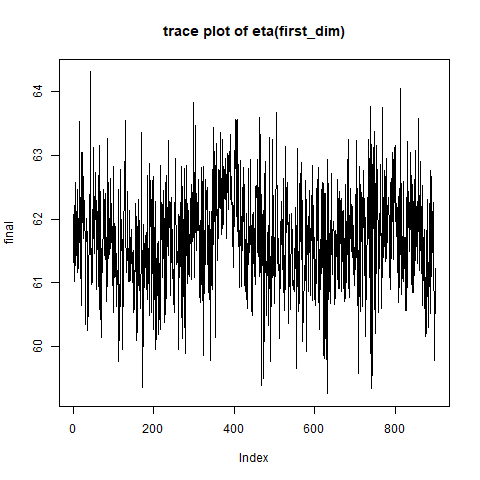
\includegraphics[width=4cm]{prob2_eta(first_dim)_traceplot.png}
    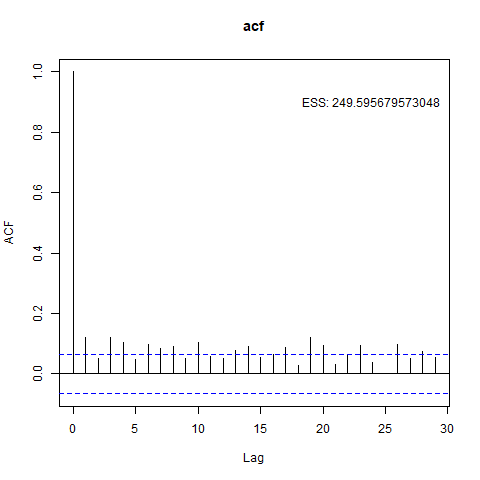
\includegraphics[width=4cm]{prob2_eta(first_dim)_acf.png}
    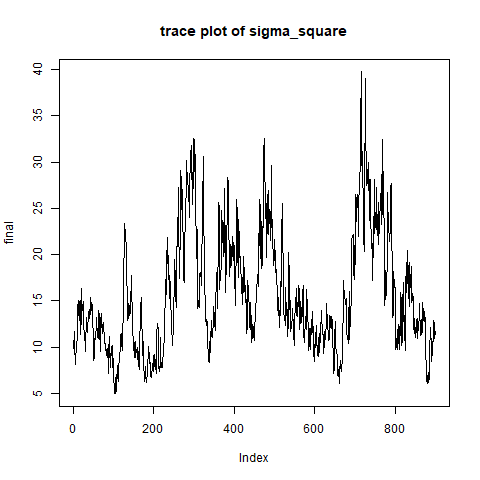
\includegraphics[width=4cm]{prob2_sigma_square_traceplot.png}
    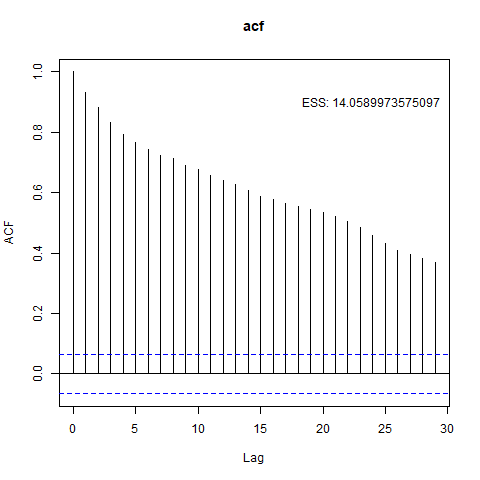
\includegraphics[width=4cm]{prob2_sigma_square_acf.png}\\
    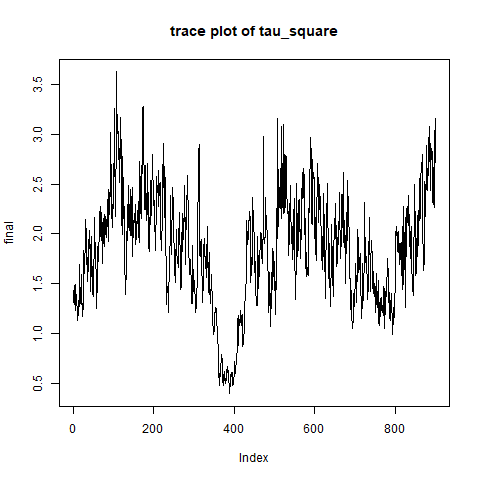
\includegraphics[width=4cm]{prob2_tau_square_traceplot.png}
    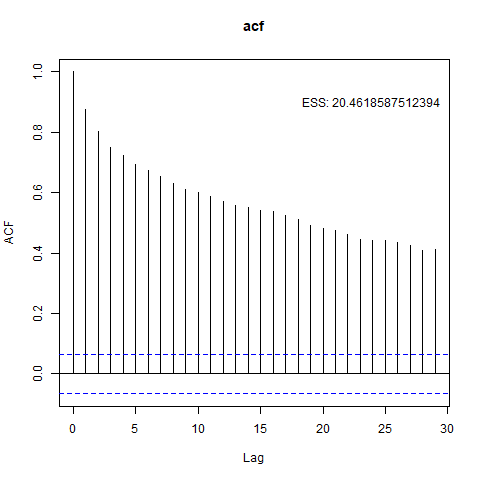
\includegraphics[width=4cm]{prob2_tau_square_acf.png}
    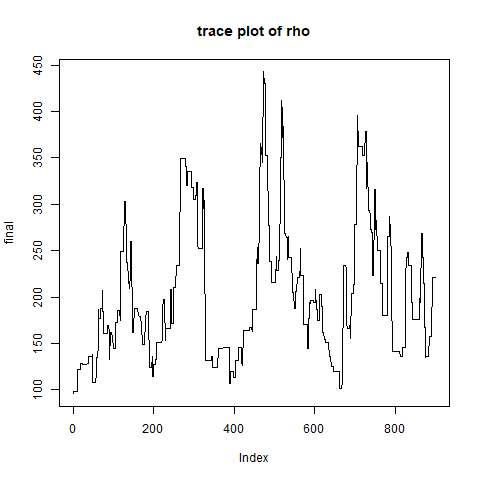
\includegraphics[width=4cm]{prob2_rho_traceplot.png}
    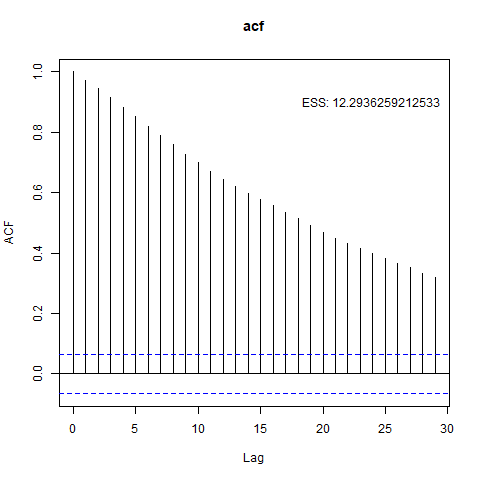
\includegraphics[width=4cm]{prob2_rho_acf.png}
    \caption{For each parameter, left:trace-plot and ESS, right:acf plot}
\end{figure}

It seems that the variance-related parameters are not mixed well. 
For better inference, we had better to run longer, cut burn-in period and do thinning.
But I stop here and report raw result of Metropolis-Gibbs sampler.

\clearpage
Finally, here are the prediction and SE plot.


\begin{figure}[!h]
    \centering
    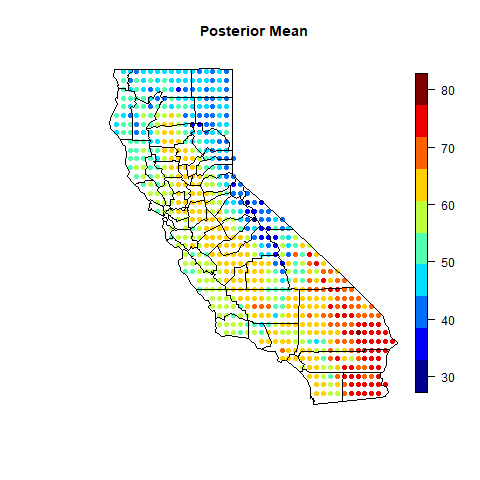
\includegraphics[height=7cm]{prob2_posterior.png}
    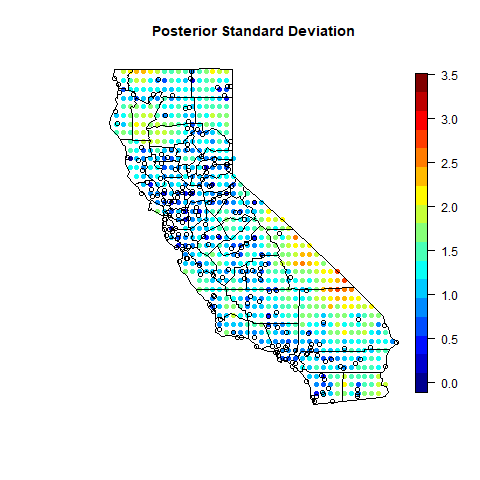
\includegraphics[height=7cm]{prob2_posterior_SE.png}
    \caption{left: prediction mean of temperature, right: standard error}
\end{figure}

Comparing these results with those of HW1, temperature values predicted by each model
are slightly different but quite similar, and both are reasonable because the results are matched 
our common sense that the temperature are inversely related to elevation, 
and directly related as going to south-east in CA region.
And Standard errors also fit to the expectation, which are higher in sparse data region than
dense data region.
Thus we conclude that the algorithm works well.


\section{Problem3}
\textbf{
Following the model in page 24 of STDA4 slide, 
implement Nimble-based MCMC code for Binomial data.
Report result for MCMC samples for $\beta,\sigma^2,\rho$ (posterior mean, traceplots, highest posterior density.)
}

I choose n, the binomial parameter, to 1 so that my model is reduced to bernoulli or binary data model.
I generate 400 data points in $[0,1]\times[0,1] \in \mathcal{R}^2\times\mathcal{R}^2$
following the GP with an exponential covariance structure (for latent variable) and bernoulli (for observable response variable).
with parameter values which I choose, $\beta_1=0, \beta1=1, \beta2=1, \sigma^2=0.1, \rho=0.1$.
And using Bayesian approach with the (normal \& inverse gamma)-GP-bernoulli hierarchical model and
MCMC algorithm provided by Nimble, get samples of posterior distributions of the parameters.

Here is a part of my R-Nimble code of declaring model and run MCMC.
I run 200,000 iterations.
\begin{Rcode}
    \begin{verbatim}
model_string = nimbleCode({

    #Data Model
    for(i in 1:n){
        prob[i] <- exp(W[i]+XB[i])/(1+exp(W[i]+XB[i]))
        Z[i] ~ dbern(prob[i])
    }
    #Constant and Cov Matrix
    XB[1:n] <- beta0*X[,1] + beta1*X[,2] + beta2*X[,3]
    covMat[1:n,1:n] <- expcov(dists[1:n,1:n],rho)
    fullCovMat[1:n,1:n] <- sigma2 * covMat[1:n,1:n]

    #Process Model
    W[1:n] ~ dmnorm(mean=mn[1:n], cov=fullCovMat[1:n,1:n])

    #Parameter Models
    sigma2 ~ dinvgamma(0.2, 0.2)
    rho ~ dunif(0,1)
    beta0 ~ dnorm(0, sd=sqrt(100))
    beta1 ~ dnorm(0, sd=sqrt(100))
    beta2 ~ dnorm(0, sd=sqrt(100))
})

niter = 200000
consts = list(n=n, X=sim_X, dists=dist_mat, mn=rep(0,n))
data = list(Z=sim_Y)
inits = list(beta0 = rnorm(1), beta1=rnorm(1), beta2=rnorm(1), rho=0.5, sigma2=2, W=rnorm(n))

pt = proc.time()
samples = nimbleMCMC(model_string, data=data, inits=inits, constants=consts,
    monitors=c("beta1","beta2","rho","sigma2","W"),
    samplesAsCodaMCMC=TRUE, WAIC=FALSE, summary=FALSE,
    niter=niter, nburnin=0, nchains=1)
ptFinal = proc.time()-pt
    \end{verbatim}
\end{Rcode}
In my computer, the elapsed time for running MCMC is 55 min 58 sec.

I cut the first 10000 samples for burn-in, and keep 190000 samples.
(In fact, I should cut more if considering the result of diagnostic plots below,
but now because I want to show you the raw result of MCMC and convergence on trace plot, 
I cut only 10000 samples.)

Below are summary things.
\begin{verbatim}
=====================================================
            beta1     beta2     sigma2     rho
true value  1         1         0.1        0.1
=====================================================
[at the sample index 10000:200000]
Mean        0.2732620 1.5722295 0.10816691 0.45473722
95%CI-Low  -0.5939745 0.7286489 0.04099271 0.02713608
95%CI-High  1.1278836 2.4583612 0.20240903 0.94366208
[at the whole sample indices]
Acc.rate    0.4395222 0.4393472 0.42739214 0.46509233
=====================================================        
\end{verbatim}

And, here are trace plots, empirical densities (role of histogram) and acf plots of
each parameter.

\clearpage
\begin{figure}[h]
    \centering
    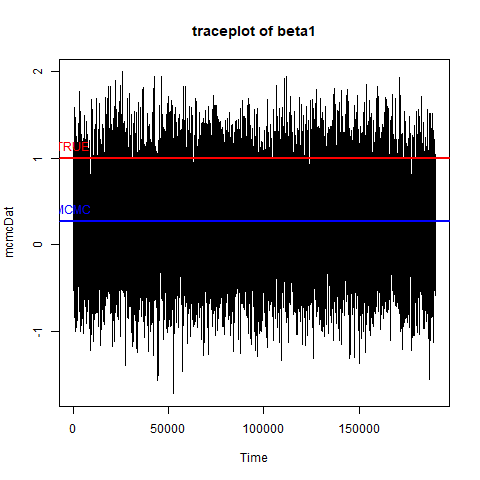
\includegraphics[width=5cm]{prob3_beta1_traceplot.png} 
    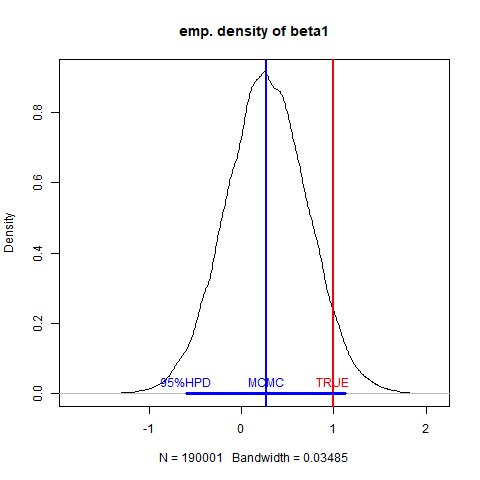
\includegraphics[width=5cm]{prob3_beta1_density.png} 
    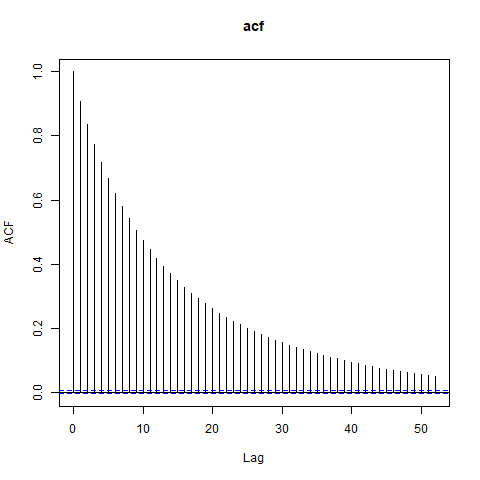
\includegraphics[width=5cm]{prob3_beta1_acf.png} \\
    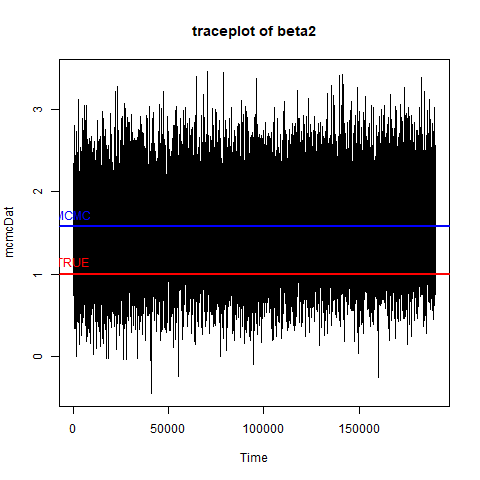
\includegraphics[width=5cm]{prob3_beta2_traceplot.png} 
    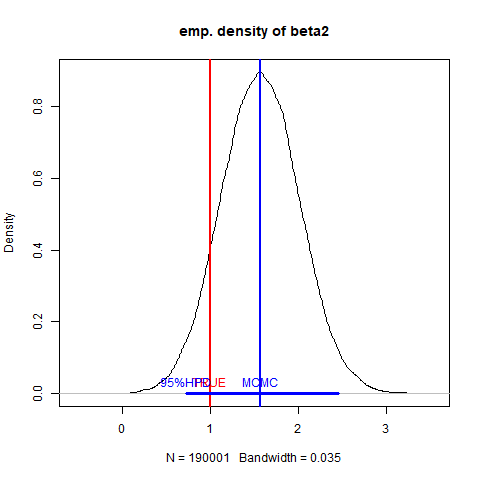
\includegraphics[width=5cm]{prob3_beta2_density.png} 
    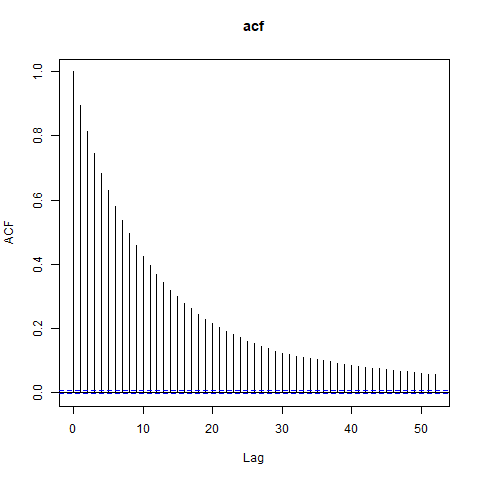
\includegraphics[width=5cm]{prob3_beta2_acf.png} \\
    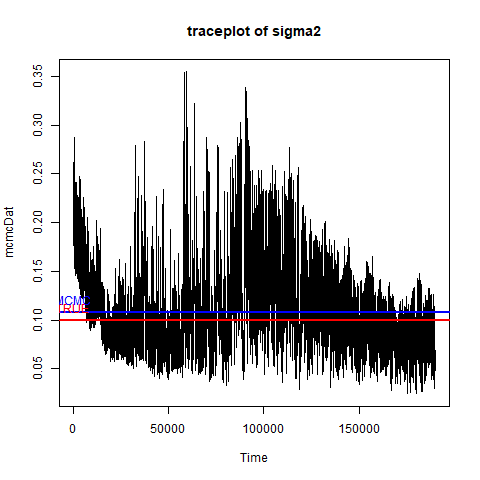
\includegraphics[width=5cm]{prob3_sigma2_traceplot.png} 
    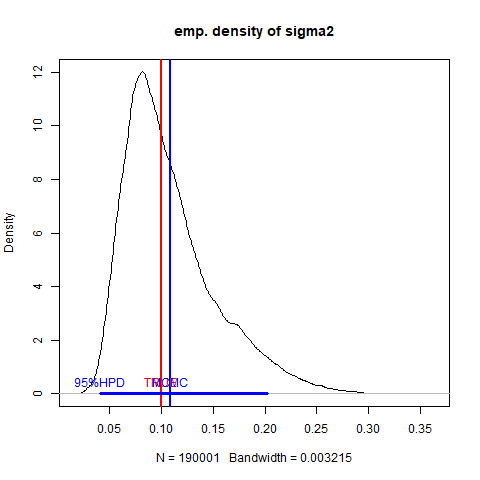
\includegraphics[width=5cm]{prob3_sigma2_density.png} 
    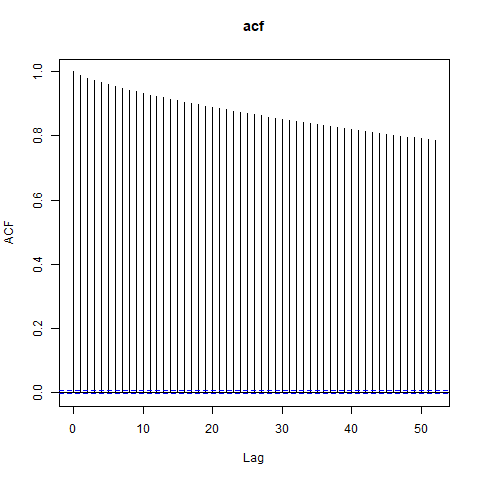
\includegraphics[width=5cm]{prob3_sigma2_acf.png} \\
    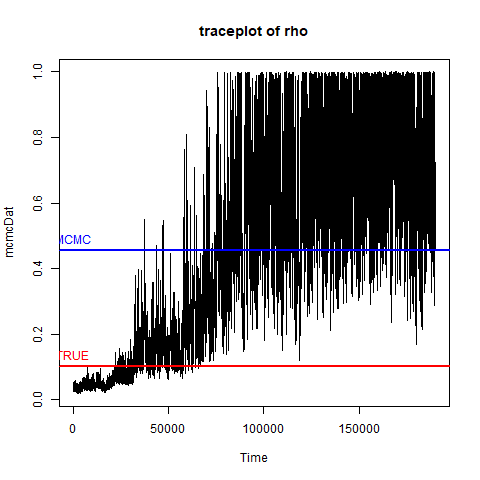
\includegraphics[width=5cm]{prob3_rho_traceplot.png} 
    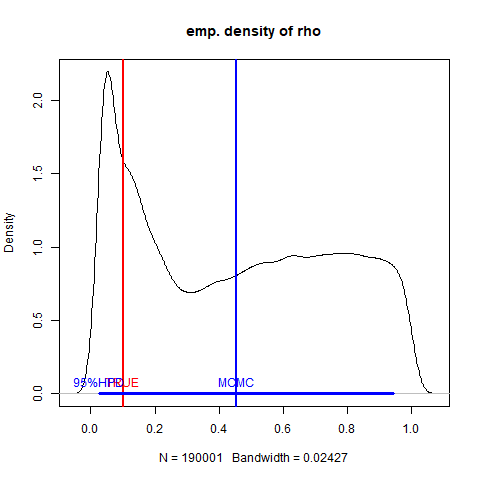
\includegraphics[width=5cm]{prob3_rho_density.png} 
    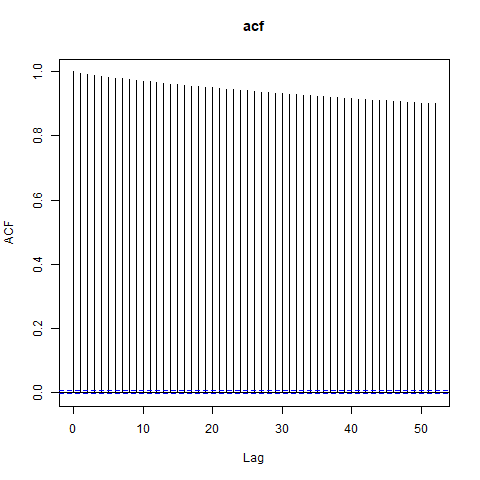
\includegraphics[width=5cm]{prob3_rho_acf.png} \\
    \caption{For each parameter, left:trace-plot, middle:sample empirical density, right:acf plot\\
    red line: true parameter value, blue line: (thin)sample mean value and (thick)95\% HPD}

\end{figure}
\clearpage

When seeing results of traceplot, $\beta$s and $\sigma^2$ converge quite well.
But you may evaluate the results as something problematic when you see 
high autocorrelation among samples, and traceplot especially of $\rho$.

In general, however, MCMC sampling from a complex distribution needs very long-iteration and
very high-level-lag thinning for proper acf. But now, I do just 200,000 iterations and don't do thinning.
If I do those additionally, the result may be better.

And in common, parameters related to variance are quite difficult to converge,
even in basic normal-normal hierarchical model. 
Thus, like our spatial model, for the cases that posterior has dependency 
or complex structure, the convergence becomes more difficult thing.
So above results, on the whole, may be admissible and tolerated.


\end{document}